\documentclass{template/custombook}
\usepackage{minted}
\usepackage{tikz}
\usepackage{titlesec}
\usepackage{biblatex}[style=ieeetr, sorting=none, backend=biber]
\addbibresource{main.bib}
\author{Dinal Atapattu}
\unitcoordinator{Dr. Matthew McKague}
\unitcode{CAB203}
\unitname{Discrete Structures}
\titleformat{\chapter}[display]
  {\normalfont\huge\bfseries}
  {\chaptername\ \thechapter} 
  {0pt}
  {\Huge}
  [\vspace{0em}]
\titlespacing*{\chapter}{0pt}{-30pt}{40pt}
\newcommand{\python}{\mintinline{python}}
\begin{document}
    \maketitle
    \tableofcontents
    \chapter{Tournament structure}
        % \section{Defining the problem instance}
        The tournament structure is defined by two constraints:
        Given the set of games as a set of pairs
        \begin{flalign}
            S = \{ (p_1, p_2), (p_3, p_4), \ldots, (p_{n-1}, p_n) \}
        \end{flalign}
        where each pair $(p_i, p_j)$ represents a game between player $p_i$ and player $p_j$.
        Using this, we can define the matches of the tournament as
        \begin{flalign}
            P = \{ u: (u,v) \in S \} \cup \{ v: (u,v) \in S \}
        \end{flalign}
        This can be modeled as the graph $G = (V, E)$ where $V = P$ and $E = S$. However, given the condition that a game between $a$ and $b$ is the same as a game between $b$ and $a$, $S$ must be symmetrised. Therefore, in order to define E, we must define a 
        symmetrising function $\mathcal{S}$ \cite{tutorial08} as follows
        \begin{flalign}
            \mathcal{S}(S) = S \cup \{ (v,u): (u,v) \in S \}
        \end{flalign}
        Using this, we can represent the set of games as
        \begin{flalign}
            E = \mathcal{S}(S)
        \end{flalign}
        As a player is unable to play against themselves, the set of games can be specified to be a \textbf{loop free undirected graph}.
        % \section{Formulating a solution}
        The constraints of the tournament structure can be defined as follows:
        \begin{enumerate}
            \item For every pair of distinct players, either they play against each other, or 
            there are at least two other players that they both play against
            \item All players have the same number of games
        \end{enumerate}
        For the first constraint, we can define the following
        \begin{flalign}
            \forall u,v \in V: \left( (u,v) \in E \wedge \left| N(u) \cap N(v)\right| \geq 2\right)
        \end{flalign}
        where $N(v)$ is the neighbour function returning the set of neighbours of a vertex. The above statement states that for all possible pairs of players, there must be an edge between them, or they must have at least two common neighbours.\\
        For the second constraint, we can define the following
        \begin{flalign}
            \left|\text{deg}(v): \forall v \in V\right| = 1 
        \end{flalign}
        where $\text{deg}(v)$ is the degree of vertex $v$. The above statement states that all players must have the same number of games.\\
        Combining the two constraints, we can define the tournament structure as
        \begin{flalign}
            \forall u,v \in V: \left( (u,v) \in E \wedge \left| N(u) \cap N(v)\right| \geq 2\right) \wedge \left|\text{deg}(v): \forall v \in V\right| = 1
        \end{flalign}
        % \section{Python Implementation}
        The python implementation utilises \mintinline{python}{set} data structures to represent the vertices and edges of the graph. A function \mintinline{python}{symmetrise(E)} implements the symmetrisation function $\mathcal{S}$, in order to symmetrise the set of edges \texttt{E}.\\
        \texttt{V} is calculated by taking every player from every edge in \texttt{E} and uses set comprehension to remove duplicates.\\
        These are then used in conjunction with a ternary operator which implements a conditional that returns false if the conditions in equation 1.5 are not met. Cardinality of sets is calculated using the \mintinline{python3}{len()} function.\\
    \chapter{Assign referees}
        We begin by modelling an instance of the problem given the CSV file.
        Each row contains a referee and their conflicts of interest in the following format
        \begin{flalign}
            R = [r_n, c_{1,1}, c_{1,2}, \ldots, c_{1,n} ] \forall R \in F
        \end{flalign}
        Where $R$ is any row excluding the header, $F$ is the CSV file, $r_n$ is a referees and $c_{1,2} \ldots c_{m,n}$ are the conflicts of interest.\\
        This data in it's current state is not useful for the task at hand. We must first parse this data in a more useful format.
        \begin{flalign}
            \intertext{Given that $P$ is the set of players, and}
            R &= \left\{ r: \left[ r,c_1,\ldots, c_n \right] \in F \right\}
        \end{flalign}
        By defining the the relationship between the referees and their conflicts of interest as 
        the function $c$, we can define the set of conflicts of interest as 
        \begin{flalign}
            c &= R \rightarrow \mathcal{P}(p)\\
            c(r) &= \left\{ c \in \mathcal{P}(p): c \in R\right\}
        \end{flalign}
        Where $\mathcal{P}(p)$ is the power set of $P$ and $c(r)$ is the set of conflicts of interest for referee $r$.
        ($[r,c_1,\ldots, c_n]$)\\
        Note that $r$ is included in the conflicts of interest as a referee cannot referee their own game.\\
        Given this, we can now formulate a solution to the problem.\\
        The task require assigning a referee to each game in the /tournament. This can be modelled as a 
        \textbf{Bipartite Graph} \cite{lecture07} \cite{lecture09} with vertices $V = G \cup R$, where
        there is a bipartition of the vertices into two sets $G$ and $R$ where $G$ is the set of games and $R$ is the set of referees (Figure \ref{fig:bipartite}).\\
        \begin{figure}[H]
            \centering
            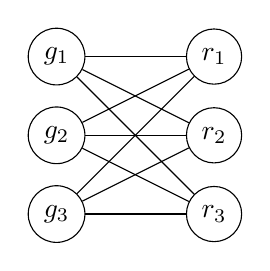
\begin{tikzpicture}
                \node[draw, circle] (g1) at (0,0) {$g_1$};
                \node[draw, circle] (g2) at (0,-1) {$g_2$};
                \node[draw, circle] (g3) at (0,-2) {$g_3$};
                \node[draw, circle] (r1) at (2,0) {$r_1$};
                \node[draw, circle] (r2) at (2,-1) {$r_2$};
                \node[draw, circle] (r3) at (2,-2) {$r_3$};
                \draw (g1) -- (r1);
                \draw (g1) -- (r2);
                \draw (g1) -- (r3);
                \draw (g2) -- (r1);
                \draw (g2) -- (r2);
                \draw (g2) -- (r3);
                \draw (g3) -- (r1);
                \draw (g3) -- (r2);
                \draw (g3) -- (r3);
            \end{tikzpicture}
            \caption{$K_{3,3}$ Bipartite graph of games and referees}
            \label{fig:bipartite}
        \end{figure}
        The assignment of a referee $r \in R$ to a game $g \in G$ will be represented as an edge between 
        a game and a referee $(r, g)$, with a valid assignment containing $|G|$ edges (one referee per game).\\
        \begin{flalign}
            E &= \left( \left\{ (g,r) : g \in G, g \cap c(r) = \emptyset \right\} \right)
        \end{flalign}
        Given the objective is to assign a referee to each game and maximising the number of valid assignments.
        This can be further defined in terms of \textbf{Maximum Matching Problem} \cite{alma991010136556004001}.
        Given the maximum matching of the graph $G = (V,E)$ as $M$, we can test the validity of this by comparing 
        the cardinality of $M$ to the cardinality of $G$. If the cardinality of $M$ is equal to the cardinality of $G$, then the matching is valid.\\
        \begin{flalign}
            \left| M \right| = \left| G \right| \implies \forall g \in G: \exists r \in R: gRr
        \end{flalign}
        Otherwise, the matching is invalid as there are games without referees.\\
        \begin{flalign}
            A = \left\{ (g,r) : g \in G, r \in R, g \cap c(r) = \emptyset \right\}
        \end{flalign}
        $A$ will be a bijective function that maps $G$ (games) to $R$ (referees) such that the referee assigned to a game is not in the conflicts of interest of the referee and every game has only one referee ($\forall g \in G : \exists r \in R: gRr$) \cite{jenner2022mxb102}\\
        This was implemented in Python by first defining the vertices \python{V} using set comprehension analogues to equation 2.1. The edges \python{E} were formed using set comprehension analogues to equation 2.7. The function $c$ defined in equation 2.4 was implemented using dictionary indexation operators on the conflicts of interest and the native Python operator \python{in} was used to confirm the presence of a referee in the conflicts of interest. The maximum matching of the graph was found using the \python{digraphs.maxMatching} function, which returned the values in a dictionary format. The validity of the matching was tested using a conditional statement that compared the cardinality of the matching to the cardinality of the games.
    \chapter{Game groups}
        Now that games have been assigned referees, we can now group games that can be played together 
        in the same time slot. However, we must first define the constraints of the problem.\\
        \begin{enumerate}
            \item People are not double-booked: each person is involved in at most one game in any game group.
            either as a player or as a referee.
            \item Games are played once. Each game is in exactly one game group
        \end{enumerate}
        This problem can easily be translated to a \textbf{Minimum Colouring Problem} \cite{discrete2012}, where the vertices are the games and referees, and the edges are the conflicts of interest, and the objective
        is to find the minimum number of colours required to colour the vertices such that no two adjacent vertices share the same colour, and to group the vertices by colour.\\
        For $((p_1, p_2), r) \in A$, where A is the set assignedReferees. This is also the set of vertices in the graph.\\
        \begin{flalign}
            V = A
        \end{flalign}
        In order to define the edges, we must first define a function that will give the set of participants/members per game
        \begin{flalign}
            \mathcal{M}((p_1, p_2), r) = \{ p_1, p_2, r \}
        \end{flalign}
        Using this we can define the set of edges as 
        \begin{flalign}
            E = \left\{ (u,v) \in V^2: \left( \mathcal{M}(u) \cap \mathcal{M}(v) \neq \emptyset \right) \wedge u \neq v \right\}
        \end{flalign}
        This gives us the graph $G = (V, E)$ where $V$ is the set of games and referees and $E$ is the set of edges.\\
        We can now obtain a minimum colouring [$c_1, c_2, \ldots, c_n$] of the edges of the graph, where $c_i$ is the colour of the $i^{th}$ edge. This will give us the game groups.

        For the Python implementation, we form the vertices \python{V} using set comprehension analogues to equation 3.1. The edges \python{E} are formed using set comprehension analgoues to equation 3.3. The function $\mathcal{S}$ defined in equation 3.2 was
        implemented using the native \python{set} function and indexation operators to extract
        the participants of a game. The colouring of the graph was found using the 
        \python{graphs.minColouring} function, which returned the values in a dictionary format.
        Which was then mapped to an array of groups of games using a dictionary comprehension 
        where the colour values were equal.
    \chapter{Game schedule}
        Given the set of assigned referees per game $A$ and the set of game groups $G$, we 
        are required to schedule each game group in a time slot such that
        \begin{itemize}
            \item People are not double-booked: each person is involved in at most one game in 
            any game group. Either as a player or referee
            \item Games are played once: each game is in exactly one game group
        \end{itemize}
        Furthermore, the committe requires the smallest number of game groups possible.\\
        Thie problem can easily be translated into a topological sorting problem, Where
        the graph $H = (V, E)$ is a \textbf{Directed Acyclic Graph (DAG)} \cite{discrete2012} \cite{lecture08}, where $V$ is the set of game groups and $E$ is the set of directed edges from a game group that must be played before another game group.\\
        \begin{flalign}
            V = G
        \end{flalign}
        In order to define the edges, we must first define a function that will give the
        assigned referee per game
        \begin{flalign}
            \mathcal{R}(g) = \{ r: (g,r) \in A \}
        \end{flalign}
        This function will give the referee assigned to a game.
        Using this we can define the set of edges as
        \begin{flalign}
            E = \left\{ (u,v) \in V^2: \left(\forall a \in u, \forall b \in v \exists a,b : \mathcal{M}(a) \cap \mathcal{R}(b) \neq \emptyset \right) \wedge u \neq v \right\}
        \end{flalign}
        This checks if there is a referee that is assigned to a game in $u$ that is also a player in a game in $v$ by checking the intersection of each element in $u$ with the referees of each element in $v$.\\
        Where $u$ precedes $v$ in the schedule. Note that an extra 
        condition is added to ensure that $u$ is not equal to $v$ to 
        avoid cycles as this would be antithetical to the nature of a DAG\cite{lecture08}.\\    
        This gives us the directed graph $H = (V, E)$ where $V$ is the set of game groups and $E$ is the set of edges running from a game group that must be played before another game group.\\
        We can now obtain a topological sorting of the graph $H$ to obtain the schedule of the game groups.\\
        By the properties of topological ordering, $u$ will always precede $v$ in the schedule if $u$ is a parent of $v$ in the graph $H$.\\
        This was implemented in Python by first defining the vertices \python{V} using set comprehension analogues to equation 4.1, each element was typecast into a \python{frozenset} in order to type errors with conventional sets due to their mutability. The edges \python{E} were formed using set comprehension analogues to equation 4.3. The function $\mathcal{R}$ defined in equation 4.2 was implemented using dictionary indexation operators on assignedReferees and 
        the native Python operator \python{in} was used to confirm the presence of a referee. The topological ordering of the graph was found using the \python{digraphs.topOrdering(V,E)}.
    \chapter{Tournament winners}
        Given the outcome of all the games in a tournament, it was required that the score be calculated and the winners be determined.\\
        Each player's maximum score is related to the primary and secondary wins that they have,
        where a primary win results in $p$ points, a secondary win 
        resulting in $s$ points. However, each secondary and primary
        win pair's points are capped at $c$.\\
        Given these constraints, we can translate this scenario to
        a \textbf{Maximum Flow Problem} where the graph $H = (V, E)$ is a directed graph where $V$ is the set of players and $E$ 
        is the set of directed edges from a winner to a loser
        The set of directed edges $E$ has been provided and is in the format $(w,l) \in E$ where $w$ is the winner and $l$ is the loser.\\ 
        Using this, we can define the vertices as the union of winners and losers
        \begin{flalign}
            V = \left\{ w: (w,l) \in E \right\} \cup \left\{ l: (w,l) \in E \right\} 
        \end{flalign}
        We must also consider the drain and source vertices for each player, this can be accounted for by the super-sink and super-source vertices which are vertices that are mapped to themselves $s$ and $t$ respectively \cite{ignjatovic_algorithms}
        \begin{flalign}
            E  = { (w,l) \in E } \cup \{ (s,s) \forall s \in V \} \cup \{ (t,t) \forall t \in V \}
        \end{flalign}
        Note that the capacities of the super source and super sink vertices are infinite.\\
        The capacity of the edges are defined by the variable $c$ which is given.\\
        As different players have different relationships with each other, 
        each graph will have different capacities for each edge.\\
        The flow of an edge is given by either the variable $p$ or $s$ depending on the type of win. Where $p$ is the primary win and $s$ is the secondary win.\\
        Primary wins are defined as the immediate out neighbours of a player, and secondary wins are defined as the out neighbours of the primary wins.\\ 
        \begin{flalign}
        \end{flalign}
    \printbibliography
\end{document}